
%(BEGIN_QUESTION)
% Copyright 2012, Tony R. Kuphaldt, released under the Creative Commons Attribution License (v 1.0)
% This means you may do almost anything with this work of mine, so long as you give me proper credit

How much tension is there in the rope where it attaches to the ceiling?

$$\includegraphics[width=15.5cm]{i02627x01.eps}$$

Also, calculate how much this suspended object weighs in units of ``pounds'', and how much mass it has in units of ``slugs''.

\vskip 10pt

Finally, calculate the mechanical advantage of this pulley system.

\underbar{file i02627}
%(END_QUESTION)





%(BEGIN_ANSWER)

Since the scale on the right-hand end of the rope registers a tension of 8 pounds, the tension at the other end of the rope must be 8 pounds as well, not counting any friction in the pulley.  All the pulley does is {\it redirect} the force pulling on the rope.

\vskip 10pt

Since the object is being supported by the tension in {\it two} rope lengths, its weight must be twice the tension:

$$W = (2) (8 \hbox{ lb}) = 16 \hbox{ lb}$$

\vskip 10pt

The relationship between mass and weight is the basic $F = ma$ formula where force $F$ is the weight of the object, $m$ is its mass, and $a$ is the acceleration of gravity:

$$m = {F \over a} = {16 \hbox{ lb} \over 32.2 \hbox{ ft/s}^2} = 0.4969 \hbox{ slugs}$$

\vskip 10pt

The mechanical advantage of any machine is (ideally) the ratio between output force and input force.  Since in this case the output force is the 16 lb weight and the input force is the 8 lb rope tension, the calculation looks like this:

$$M_A = {F_{out} \over F_{in}}$$

$$M_A = {16 \hbox{ lb} \over 8 \hbox{ lb}} = 2$$

In other words, for every pound of force applied on the rope, there will be 2 pounds of force available to move the mass.

%(END_ANSWER)





%(BEGIN_NOTES)


%INDEX% Machine, pulley
%INDEX% Machine, mechanical advantage

%(END_NOTES)


